\chapter{Architecture}

In this section, we discuss the architectural advancement on top of the original Plasticine architecture
introduced in~\cite{plasticine}. These architectural additions helps increase the application
coverage or improve the mapping strategies of existing applications by supporting new language
constructs, data types, and improves the utilizations of the hardware. 
Specifically, \Cref{sec:banking_arch} lay outs the datapath changes in order to support more
flexible banking schemes required by general access patterns supported in Spatial; 
\Cref{sec:rnn_arch} discusses the hardware specialization and architectural sizing for machine
learning applications; \Cref{network} provides an extensive study on on-chip network selection 
reconfigurable spatial architectures.

\begin{figure*}
\centering
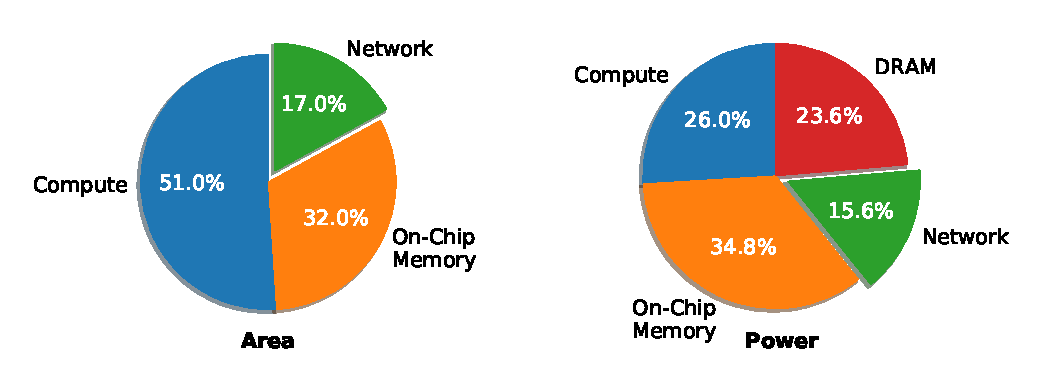
\includegraphics[width=1\textwidth]{figs/pie.pdf}
\caption[Area and power breakdown of Plasticine]{
  Area and power breakdown of Plasticine
}
\label{fig:breakdown}
\end{figure*}
